\chapter{Caminhos em Grafos}

\section{Caminhos em Redes Estáticas}
Dentre os diversos problemas que surgem em grafos, este é o mais fundamental de todos e
aquele que ao longo dos anos foi dos mais estudados. Várias técnicas surgiram desde os meados
de 1950 com o objetivo de tratar eficientemente o problema de caminhos mínimos em grafos. A
principal delas considera o fato de se promover uma arborescência em um grafo onde a medida
que os vértices explorados são atingidos, tem-se uma proximidade da solução do problema \cite{negreirosbook}.

\subsection{Problema de Caminho Mínimo}
Uma rede de transporte (que pode ser uma malha viária, rodoviária, etc.) pode ser
representada por uma grafo $G = (N, A)$, onde $N$ é o conjunto de nós e A é o conjunto de arcos
os quais interligam estes nós. Considerado o número de nós $|N| = n;$ e o número de arcos $|A| = m;$ para
cada arco $(i, j) \in A$ está associado um custo unitário $c_{ij}$. O caminho entre um
nó origem $(s)$ e um nó destino $(t)$ é definido por uma sequência de
arcos: $(s,i),...(k,l),...(j,t)$. O Problema de Caminho Mínimo (PCM) consiste em determinar
um caminho entre $s$ e $t$ tal que a somatória dos custos unitários dos arcos (ou alguma
outra medida de impedância) que compõem este caminho seja o mínimo \cite{cunha}.

Dada uma rede $G$ com $m$ nós e $n$ arcos, associando a cada arco $(i,j)$ o custo $c_{ij}$, o Problema
de Caminho Mínimo é encontrar o menor caminho entre o nó 1 para o nó $m$ em $G$ (caminho mínimo de menor valor).
O custo do caminho é a soma dos custos sobre os arcos do caminho encontrado. Uma formatação genérica do problema
de caminho mínimo é dada via grafos, quando deseja-se encontrar o percurso de custo mínimo entre dois vértices $i$ e $j$
de um grafo $G(V,L)$, onde, se $\exists$ $\Gamma (i,j)$, $i$, $j \in V$, então $w_{ij}$ é tomado como o custo mínimo
de um caminho direto entre os vértices $i$ e $j$, e todo $i_1$, ..., $i_k \in V$, distintos de $i$, $j$, são ditos
serem vértices do caminho, onde $i$ precede $i_1$ e assim por diante, nesta ordem \cite{negreirosbook}.

O princípio de qualquer algoritmo de caminho mínimo está associado ao seguinte teorema demonstrado 
em \cite{negreirosbook}, como mostra a figura \ref{fig:teorema}:

$C(\Gamma(s,t)) = C(\Gamma(s,k)) + C(\Gamma(k,t))$ é mínimo $\Longleftrightarrow$ $\Gamma(s,k)$ é mínimo e $\Gamma(k,t)$ é mínimo.

\begin{figure}[htbp]
\centering
 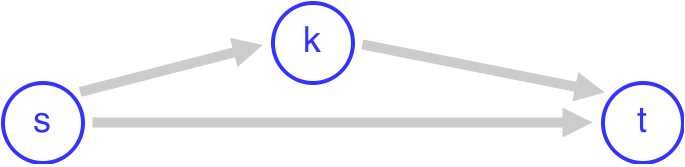
\includegraphics[width=.45\textwidth]{chapters/fig/teorema.png}
\caption{Teorema - Princípio do algoritmo de caminho mínimo}
\label{fig:teorema}
\end{figure}
\FloatBarrier

% \newtheorem{meuteorema}{Teorema}[chapter]
% \begin{meuteorema} \label{teo:Pita} 
% Supondo $k$ um nó intermediário de um caminho de peso mínimo $\Gamma_c$.
% Então o subcaminho $\Gamma_k$ de $\Gamma_c$ é um caminho de peso mínimo de $\Gamma_k$.
% \end{meuteorema}
% \begin{proof} (Contradição)
% Seja ...
% \end{proof}


\subsection{Algoritmo de Dijkstra}
O algoritmo de Dijkstra foi proposto em 1959 e permite determinar a solução ótima através da adição de
vértices à árvore de caminho mínimo pelo processo de relaxamento de uma aresta, que consiste em verificar
se há a possibilidade de melhorar o caminho obtido até o momento \cite{boaventura}. Este algoritmo considera
basicamente um processo de rotulação de vértices à medida que o mínimo caminho é encontrado passo a passo,
interativamente, em vértices intermediários. O algoritmo requer que nenhum peso no grafo seja negativo. Abaixo
é apresentado o pseudocódigo do algoritmo de Dijkstra.
\FloatBarrier
\fbox{\begin{minipage}{70ex}
\noindent \phantom{} \hspace{0ex} {\bf AlgoritmoDijkstra}\\
\vspace*{-1mm} \phantom{} \hspace{3ex} inicialize a distância para todos os nós em G = infinito\\
\vspace*{-1mm} \phantom{} \hspace{3ex} inicialize o predecessor de todos os nós em G = vazio\\
\vspace*{-1mm} \phantom{} \hspace{3ex} {\bf Enquanto} H não estiver vazio faça\\
\vspace*{-1mm} \phantom{} \hspace{6ex} u = o nó com menor rótulo extraído de H\\
\vspace*{-1mm} \phantom{} \hspace{6ex} {\bf Para} cada v adjacente a u:\\
\vspace*{-1mm} \phantom{} \hspace{9ex} {\bf Se} rótulo[v] > rótulo[u] + distância[u, v]:\\
\vspace*{-1mm} \phantom{} \hspace{12ex} rótulo[v] = rótulo[u] + distância[u, v];\\
\vspace*{-1mm} \phantom{} \hspace{12ex} predecessor[v] = u;\\
\vspace*{-1mm} \phantom{} \hspace{12ex} atualiza a posição de v em H\\
\vspace*{-1mm} \phantom{} \hspace{9ex} {\bf Fim Se}\\
\vspace*{-1mm} \phantom{} \hspace{6ex} {\bf Fim Para}\\
\vspace*{-1mm} \phantom{} \hspace{3ex} {\bf Fim Enquanto}\\
\vspace*{-1mm} \phantom{} \hspace{0ex} {\bf Fim Dijkstra}\\
\end{minipage}}
\begin{figure}[htbp]
\centering
\caption{Algoritmo de Dijkstra}
Fonte: \cite{cormen}
\label{fig:codeRadix}
\end{figure}

% \begin{center}
%   \line(1,0){450}
% \end{center}
% \lstinputlisting[language=Java]{chapters/dijkstra.js}
% \begin{figure}[htbp]
%   \begin{center}
%     \line(1,0){450}
%   \end{center}
%   \centering
%   \caption{Estrutura JSON usada pelo Dynagraph}
%   \label{fig:jsondyn}
% \end{figure}

\subsection{Algoritmo Radix Heap}
O algoritmo Radix Heap é utilizado numa variação do algoritmo de Dijkstra e foi proposto inicialmente por
Ahuja, Mehlhorn, Orlin e Tarjan em \cite{ahuja}.
Ele é considerado ainda no meio científico como um dos algoritmos mais eficientes para resolver o
problema do caminho mínimo.
A implementação do Radix Heap é um híbrido da implementação primitiva $O(n^2)$ e implementação de Dial($O(m + nC))$). 
Estas duas implementações representam dois extremos no que diz respeito à quantidade dos buckets utilizados.
A implementação primitiva considera todos os vértices rotulados temporariamente juntos, em um bucket grande,
e procura por um vértice com o menor rótulo. Já o algoritmo de Dial usa um grande número de buckets e separa os vértices,
armazenando dois vértices quaisquer com rótulos diferentes em diferentes segmentos \cite{bookahuja}.
A implementação Radix Heap melhora esses dois métodos através de uma solução intermediária:
Ele armazena vários, mas não todos os vértices em um mesmo bucket. Por exemplo, em vez de armazenar
apenas os vértices com $d[v] = k$ em um bucket k, como na implementação do Dial,
pode-se armazenar todos os vértices com $d[v]$ dentro do intervalo [100$k$ para 100$k$ + 99] no bucket $k$ \cite{bookahuja}.

Para o bucket[k] é definido um intervalo de valores denotado por intervalo(k). O número de inteiros
no intervalo é chamado de largura do intervalo e denotado por largura(k).
No exemplo anterior, o intervalo do bucket $k$ é [100$k$, 100$k$ + 99] e sua largura é 100. 

Usar larguras de tamanho $k$ permite reduzir o número de buckets necessários por um fator de $k$.
Mas para encontrar o rótulo de menor distância, é preciso procurar todos os elementos no bucket não vazio de menor índice.
Para superar isso, o algoritmo radix heap considera usar larguras variáveis e altera os intervalos de forma dinâmica. 
O Radix Heap segue as propriedades:

1. As larguras dos buckets são 1, 1, 2, 4, 8, 16, ..., de modo que o número de buckets necessários é somente $O(log(NC))$,
onde N é o número de vértice e C o custo da maior aresta.

2.  Os intervalos dos buckets são modificados dinamicamente e são realocados os vértices de menor rótulo temporário
para um único bucket, cuja largura é 1.

A Propriedade 1 nos permite manter apenas $O(log(NC))$ buckets e, assim, supera a desvantagem do algoritmo
de Dial, que usa muitos buckets.
A Propriedade 2 nos permite, como no algoritmo Dial, evitar a necessidade de 
pesquisar todo o bucket para encontrar um vértice de menor rótulo temporário. Quando implementado deste modo, esta 
versão do algoritmo radix heap tem complexidade $O(m + nlog(nC))$ \cite{bookahuja}.

Para um dado problema de caminho mínimo, o radix heap consiste em $1 + [log(NC)]$ buckets.
Os buckets são numeradas de $0$ até $K = [log(nC)]$.
O algoritmo irá alterar os intervalos dos buckets de forma dinâmica, e cada vez que muda os intervalos,
redistribui os vértices nos buckets. Inicialmente, os buckets têm os seguintes intervalos:\\
intervalo(0) = [0];\\
intervalo(1) = [1];\\
intervalo(2) = [2, 3];\\
intervalo(3) = [4, 7];\\
intervalo(4) = [8, 15];\\
...\\
intervalo(K) = [$2^{K - 1}$, $2^K - 1$].

Esses intervalos mudam à medida que o algoritmo prossegue. No entanto, a largura dos buckets nunca aumenta
para além das suas larguras iniciais \cite{bookahuja}.

\subsubsection{Operações sobre o Radix Heap}
Determinar qual intervalo contém um dado valor pode ser feito percorrendo o vetor de buckets com complexidade $O(lognC)$.
Logo, inserir um vértice na estrutura, tem complexidade $O(K)$, pois $O(K) = O(lognC)$

Para descrever a operação de retirar o item da fila de prioridades que contém o menor valor chave considere o seguinte exemplo:
Supondo que o rótulo temporário de um vértice de conteudo(4) é 9, cujo intervalo é [8, 15].
O algoritmo irá examinar cada vértice em conteudo(4) para identificar um vértice com o rótulo de menor distância.
Segundo \cite{bookahuja}, os rótulos de distância que o algoritmo de Dijkstra designa como permanente não são decrescentes,
isso implica que nenhum rótulo temporário de distância jamais voltará
a ser inferior a 9 e, consequentemente, não precisará mais dos buckets de 0 a 3.

Em vez de deixar estes buckets inativos, o algoritmo redistribui o intervalo[9, 15]
para os buckets anteriores, resultando nos intervalos intervalo(0) = [9], intervalo(1) = [10],
intervalo(2) = [11, 12], intervalo(3) = [13,15] e intervalo(4) = $\emptyset$ . Uma vez que o intervalo(4)
está vazio agora, o algoritmo redistribui os vértices que estavam em conteudo(4) para os buckets adequados (0, 1, 2, e 3).
Assim, cada um dos vértices no bucket 4 move-se para um bucket de menor índice e todos vértices com o rótulo de menor distância
são movidos para o bucket 0, que tem largura 1 \cite{bookahuja}.

\subsubsection{Funcionamento do Algoritmo de Dijkstra com Radix Heap}
Sempre que o algoritmo encontra vértices com o rótulo de menor distância em um bucket com
largura maior que 1, ele verifica todos os vértices no bucket para identificar um vértice com rótulo de menor distância.
Em seguida, o algoritmo redistribui o intervalo dos buckets e muda cada vértice no bucket para o bucket de menor índice.
Uma vez que o radix heap contém $k$ buckets, um vértice pode mudar na maioria das $k$ vezes, e consequentemente,
o algoritmo irá verificar qualquer vértice na maioria das $k$ vezes. Por isso, o número total de verificações
de vértices é $O(NK)$, o qual não é "muito grande" \cite{bookahuja}.

Para demonstrado o funcionamento do algoritmo de Dijkstra com Radix Heap serão utilizadas figuras do livro \cite{bookahuja}.
O grafo na figura \ref{fig:grafoRadix} exemplifica o radix heap, e o número ao lado de cada arco indica o seu comprimento.
\FloatBarrier
\begin{figure}[htbp]
\centering
 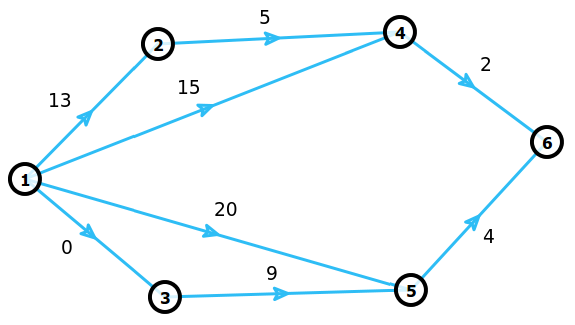
\includegraphics[width=.65\textwidth]{chapters/fig/grafoRadix.png}
\caption{Grafo - Caminho Mínimo}
\label{fig:grafoRadix}
\end{figure}
\FloatBarrier
O vértice origem é $s = 1$. O peso da maior aresta é $C = 20$, logo $K = [log(nC))] = [log(120)] = 7$.
A Tabela \ref{tab:initialradixheap} especifica os rótulos de distância determinada pelo algoritmo de Dijkstra
após análise do vértice 1.
\FloatBarrier
\begin{table}[htbp]
	\centering
	\begin{tabular}{l l l l l l l}
	\toprule
	vértice $i$ & 1 & 2 & 3 & 4 & 5 & 6\\
	\midrule
	rótulo d[$i$] & 0 & 13 & 0 & 15 & 20 & $\infty$ \\
	\bottomrule
	\end{tabular}
	
	\centering
	\begin{tabular}{l l l l l l l l l}
	\toprule
	\\bucket $k$ & 0 & 1 & 2 & 3 & 4 & 5 & 6 & 7\\
	\midrule
	\\intervalo($k$) & [0] & [1] & [2, 3] & [4, 7] & [8, 15] & [16, 31] & [32, 63] & [64, 127]\\
	\\conteudo($k$) & \{3\} & $\emptyset$ & $\emptyset$ & $\emptyset$ & \{2, 4\} & \{5\} & $\emptyset$ & \\
	\bottomrule
	\end{tabular}
\caption{Radix Heap inicial}
 \label{tab:initialradixheap}
\end{table}

Para selecionar o vértice com o rótulo de menor distância, os buckets 0, 1, 2, ..., K são percorridos para encontrar o
primeiro bucket não vazio. No exemplo, o bucket 0 é não vazio. Uma vez que o bucket 0 tem largura 1,
cada vértice neste bucket tem o mesmo (no mínimo) rótulo de distância. Assim, o algoritmo determina o vértice 3 como permanente,
exclui o vértice 3 do radix heap, e verifica o arco (3, 5) para alterar o rótulo de distância do vértice 5 de 20 para 9.
Em seguida, é verificado se o novo rótulo de distância do vértice 5 está contido no intervalo de seu bucket presente,
que é o bucket 5. Como o seu rótulo de distância diminuiu, o vértice 5 deve se mover para um bucket de menor índice.
Assim, é concluída a análise sequencial dos bucket da direita para a esquerda, a partir do bucket 5,
para identificar o primeiro bucket cujo intervalo contém o número 9, que é o bucket 4.
O vértice 5 é movido do bucket 5 para bucket 4. A tabela \ref{tab:secondradixheap} mostra o novo radix heap.

\begin{table}[htbp]
	\centering
	\begin{tabular}{l l l l l}
	\toprule
	vértice $i$ & 2 & 4 & 5 & 6\\
	\midrule
	rótulo d[$i$] & 13 & 15 & 9 & $\infty$ \\
	\bottomrule
	\end{tabular}
	
	\centering
	\begin{tabular}{l l l l l l l l l}
	\toprule
	\\bucket $k$ & 0 & 1 & 2 & 3 & 4 & 5 & 6 & 7\\
	\midrule
	\\intervalo($k$) & [0] & [1] & [2, 3] & [4, 7] & [8, 15] & [16, 31] & [32, 63] & [64, 127]\\
	\\conteudo($k$) & $\emptyset$ & $\emptyset$ & $\emptyset$ & $\emptyset$ & \{2, 4, 5\} & $\emptyset$ & $\emptyset$ & $\emptyset$\\
	\bottomrule
	\end{tabular}
\caption{Radix Heap - final da iteração 1}
 \label{tab:secondradixheap}
\end{table}
\FloatBarrier
Varrendo os buckets sequencialmente, é observado que o bucket $k = 4$ é o primeiro bucket não vazio.
Uma vez que o intervalo deste bucket contém mais de um número inteiro, o primeiro vértice no bucket não precisa ter
o rótulo de menor distância. Tem-se que intervalo(4) é [8, 15], mas como seu menor rótulo temporário neste bucket é 9,
o novo intervalo a ser redistribuído é intervalo[9, 15] da seguinte maneira:\\
intervalo(0) = [9],\\
intervalo(1) = [10],\\
intervalo(2) = [11, 12],\\
intervalo(3) = [13, 15],\\
intervalo(4) = $\emptyset$.

Outros intervalos não mudam. Os vértices do bucket 4 foram redistribuídos nos buckets 0 a 3.
Os buckets resultantes têm os seguintes conteúdo:\\
conteúdo(0) = {5},\\
conteúdo(1) = $\emptyset$,\\
conteúdo(2) = $\emptyset$,\\
conteúdo(3) = {2, 4},\\
conteúdo(4) = $\emptyset$.

Esta redistribuição esvazia necessariamente o bucket 4 e move o vértice com o rótulo de menor distância para o bucket 0.

\subsubsection{Complexidade do Algoritmo de Dijkstra com Radix Heap}
Cada operação de inserção do vértice no bucket consome tempo $O(K)$.
Como um vértice só pode ser movido $K$ vezes no máximo, então $O(nK)$ é um limite para o número total de movimentos
de vértices.
O termo $m$ significa o número de distâncias atualizadas, logo o tempo total gasto em atualizar os rótulos temporários
é $O(m + nK)$.
A operação de selecionar um vértice começa verificando os buckets da esquerda para a direita para encontrar
o primeiro bucket não vazio $k$ no radix heap. Esta operação requer tempo $O(K)$ por iteração e $O(nk)$ no total.
A redistribuição do intervalo segue atribuindo o primeiro inteiro para bucket 0, o próximo inteiro para bucket 1,
os próximos dois inteiros para bucket 2, nos próximos quatro inteiros para bucket 3, e assim por diante.
Uma vez que o bucket $k$ tem uma largura inferior a $2^{k - 1}$, e uma vez que as larguras dos primeiros $k$ buckets
pode ser tão grande como $1, 1, 2, ..., 2^{k - 2}$ até uma largura total de potencial $2^{k - 1}$,
o intervalo útil do bucket k sobre os buckets $0, 1, ..., k - 1$ é redistribuído.
Esta redistribuição dos intevalos e re-inserções subsequentes de vértices esvazia o bucket k e move os vértices com
os rótulos de menor distância para o bucket 0 \cite{bookahuja}.
Portanto, como $k = [log(nC)]$, o tempo de execução do algoritmo de Dijkstra com Radix Heap é $O(m + nk) = O(m + n log(nC))$.
Usando a estrutura de dados Fibonacci heap com a implementação do radix heap, é possível reduzir ainda mais a complexidade
para $O(m + n\sqrt{logC})$, o que dá uma execução mais rápida do algoritmo em tempo polinomial para resolver
o problema do caminho mínimo com comprimentos de arcos não negativos \cite{ahuja}.
A Figura \ref{fig:codeRadix} apresenta o pseudocódigo do algoritmo Radix Heap.

\fbox{\begin{minipage}{70ex}
\vspace*{-1mm} \phantom{} \hspace{0ex} {\bf AlgoritmoRadixHeap}\\
\vspace*{-1mm} \phantom{} \hspace{3ex} buckets = [];\\
\vspace*{-1mm} \phantom{} \hspace{3ex} distancias = [];\\
\vspace*{-1mm} \phantom{} \hspace{3ex} Inicializa o rótulo de distância dos vértices\\
\vspace*{-1mm} \phantom{} \hspace{3ex} {\bf Para} i = 1 até i < vertices.length\\
\vspace*{-1mm} \phantom{} \hspace{6ex} distancias[i] = MAXINT\\
\vspace*{-1mm} \phantom{} \hspace{3ex} {\bf Fim Para}\\
\vspace*{-1mm} \phantom{} \hspace{3ex} Inicializa os buckets e seus intervalos\\
\vspace*{-1mm} \phantom{} \hspace{3ex} {\bf Para} i = 0 até i < buckets.length\\
\vspace*{-1mm} \phantom{} \hspace{6ex} iniBucket = $2^{k - 1}$\\
\vspace*{-1mm} \phantom{} \hspace{6ex} fimBucket = $2^k - 1$\\
\vspace*{-1mm} \phantom{} \hspace{3ex} {\bf Fim Para}\\
\vspace*{-1mm} \phantom{} \hspace{3ex} Insere os vértices dentro dos buckets correspondentes\\
\vspace*{-1mm} \phantom{} \hspace{3ex} {\bf Enquanto} todos os vértices não forem rotulados permanentemente\\
\vspace*{-1mm} \phantom{} \hspace{6ex} menorBucket = menor bucket não vazio\\
\vspace*{-1mm} \phantom{} \hspace{6ex} {\bf Se} (o menorBucket tem largura = 1 || menorBucket.size = 1)\\
\vspace*{-1mm} \phantom{} \hspace{9ex} verticeSelecionado = vértice do menorBucket\\
\vspace*{-1mm} \phantom{} \hspace{9ex} {\bf Para} i = 0 até i < número de arcos do verticeSelecionado\\
\vspace*{-1mm} \phantom{} \hspace{12ex} Atualiza o rótulo de distância dos vértices\\
\vspace*{-1mm} \phantom{} \hspace{12ex} Insere o vértice no bucket que contenha a sua faixa de valores\\
\vspace*{-1mm} \phantom{} \hspace{9ex} {\bf Fim Para}\\
\vspace*{-1mm} \phantom{} \hspace{9ex} Remove do heap o verticeSelecionado\\
\vspace*{-1mm} \phantom{} \hspace{9ex} Marca o rótulo verticeSelecionado como permanentemente\\
\vspace*{-1mm} \phantom{} \hspace{6ex} {\bf Fim Se}\\
\vspace*{-1mm} \phantom{} \hspace{6ex} {\bf Senão}\\
\vspace*{-1mm} \phantom{} \hspace{9ex} Recalcula o intervalo dos buckets\\
\vspace*{-1mm} \phantom{} \hspace{9ex} Redistribui os vertices\\
\vspace*{-1mm} \phantom{} \hspace{3ex} {\bf Fim Enquanto}\\
\vspace*{-1mm} \phantom{} \hspace{0ex} {\bf Fim RadixHeap}\\
\end{minipage}}
\begin{figure}[htbp]
\centering
\caption{Radix Heap - Pseudocódigo do algoritmo}
\label{fig:codeRadix}
\end{figure}
\FloatBarrier

\section{Caminhos em Redes Dinâmicas}
\label{sec:pathdyn}
Embora o Problema de Caminho Mínimo seja um dos problemas de otimização combinatória mais bem estudados
na literatura \cite{bookahuja}, Caminhos em Redes Dinâmicas tem recebido muito menos atenção ao longo dos anos.
\cite{giacomo} aborda duas categorias de Problema de Caminho Mínimo em Grafos Dinâmicos. O primeiro é chamado
geralmente na literatura de variante dependente do tempo: o custo de um arco é o tempo de viagem, que é dado
por uma função pré-determinada de tempo, que significa que o custo de um arco $(u, v)$ sobre um caminho
depende do tempo a partir do caminho e do tempo já gasto para alcançar $u$.
O segundo ainda não tem um nome comum na literatura: são grafos onde a função de custo muda ou é atualizada
depois de um certo intervalo de tempo, mas o grafo é estático entre duas alterações da função custo.

\subsection{Algoritmos de Caminho Mínimo Dinâmico}
Essa seção aborda 3 tipos de estruturas:
\begin{itemize}
\item Topologia Estática e Atributos Dinâmicos;
\item Topologia Dinâmica e Atributos Estáticos;
\item Topologia Dinâmica e Atributos Dinâmicos.
\end{itemize}

\subsubsection{Topologia Estática e Atributos Dinâmicos}
\label{subsec:limitesuperior}
\cite{leonard} trata o Problema de Caminho Mínimo com previsão de tempo utilizando um vetor de custos e
através da aplicação do algoritmo Dijkstra modificado. O vetor de custos é composto por dados das passagens 
dos veículos na via como instante da passagem, velocidade, tipo e placa do veículo, que são periodicamente calculados
a cada 10 minutos para cada ligação ou aresta. O algoritmo de Dijkstra é modificado para que o mesmo atualize os custos
de suas arestas à medida que os tempos de percurso se modificam, pois o trânsito dos veículos nas vias descreve um
comportamento dinâmico ao longo do tempo.

Por exemplo, se o tempo parcial até um determinado ponto for de 7 minutos, então
é utilizado para o próximo cálculo o tempo de previsão no intervalo $t + 1$, mas se o tempo parcial for de 15 minutos, logo
o período de previsão é ultrapassado, e com isso utiliza-se $t + 2$ para o cálculo do próximo trajeto. Se o tempo parcial
estiver entre 30 e 40 minutos utiliza-se o intervalo $t + 4$, entre 40 e 50 minutos $t + 5$, e assim por diante.
Essa abordagem só altera o intervalo de previsão quando o valor do custo do vértice for superior a 10.
A figura \ref{fig:diMod} apresenta o pseudocódigo do algoritmo Dijkstra Modificado.

\fbox{\begin{minipage}{70ex}
\noindent \phantom{} \hspace{0ex} {\bf Algoritmo Dijkstra Modificado}\\
\vspace*{-1mm} \phantom{} \hspace{0ex} Início\\
\vspace*{-1mm} \phantom{} \hspace{3ex} inicialize a distância para todos os nós em G = infinito\\
\vspace*{-1mm} \phantom{} \hspace{3ex} inicialize o predecessor de todos os nós em G = vazio\\
\vspace*{-1mm} \phantom{} \hspace{3ex} {\bf Enquanto} H não estiver vazio faça\\
\vspace*{-1mm} \phantom{} \hspace{6ex} u = o nó com menor rótulo extraído de H\\
\vspace*{-1mm} \phantom{} \hspace{6ex} {\bf Para} cada v adjacente a u:\\
\vspace*{-1mm} \phantom{} \hspace{9ex} {\bf Se} rótulo[v] > rótulo[u] + distância[u, v][t]:\\
\vspace*{-1mm} \phantom{} \hspace{12ex} rótulo[v] = rótulo[u] + distância[u, v][t];\\
\vspace*{-1mm} \phantom{} \hspace{12ex} predecessor[v] = u;\\
\vspace*{-1mm} \phantom{} \hspace{12ex} atualiza a posição de v em H\\
\vspace*{-1mm} \phantom{} \hspace{9ex} {\bf Fim Se}\\
\vspace*{-1mm} \phantom{} \hspace{6ex} {\bf Fim Para}\\
\vspace*{-1mm} \phantom{} \hspace{3ex} {\bf Fim Enquanto}\\
\vspace*{-1mm} \phantom{} \hspace{0ex} {\bf Fim Dijkstra}\\
\end{minipage}}
\begin{figure}[htbp]
\centering
\caption{Dijkstra Modificado - Pseudocódigo do algoritmo}
\label{fig:diMod}
\end{figure}
\FloatBarrier

A seguir, é apresentado o funcionamento do algoritmo. O exemplo na figura \ref{fig:leo1} utiliza
6 pontos representados através do grafo G(N=\{P1, P2, P3, P4, P5, P6\}, A).

\begin{figure}[htbp]
\centering
 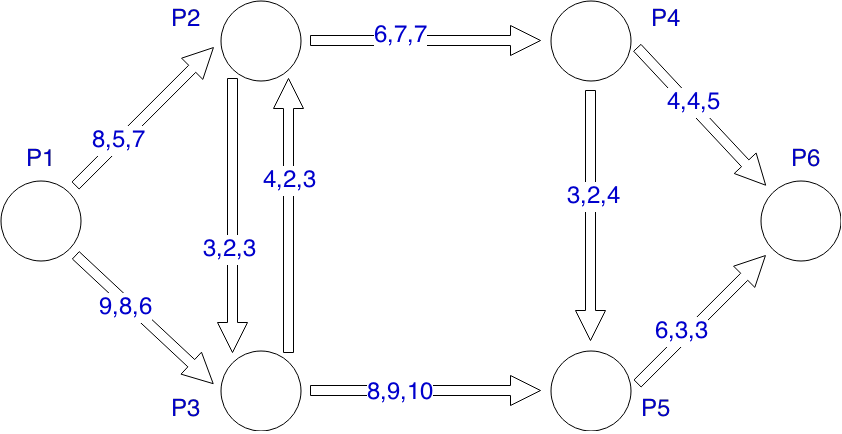
\includegraphics[width=.60\textwidth]{chapters/fig/leo1.png}
\caption{Grafo exemplo para determinação de caminho mínimo}
Fonte: Elaboração própria, baseada em \cite{leonard}
\label{fig:leo1}
\end{figure}

As arestas possuem vários pesos que são os tempos de percursos previstos entre os pontos para os tempos
futuros $t + 1$, $t + 2$ e $t + 3$. Esses custos são armazenados no algoritmo através de um vetor de atributos.
Para determinar o caminho mínimo, utiliza-se um conjunto chamado PERM, que inicialmente contém o vértice fonte P1.
A qualquer momento PERM contém todos os vértices para os quais já foram determinados os menores caminhos usando
apenas vértices em PERM, a partir de P1. Para cada vértice $s$ fora de PERM mantém-se a menor distância dentro do
seu respectivo intervalo de previsão dist[$s$] de P1 a $s$ usando caminhos onde o único vértice que não está em
PERM seja $s$ \cite{leonard}.

Outra característica do algoritmo é a necessidade de armazenar o vértice adjacente
a $s$ neste caminho em path[$s$]. Selecionando o vértice com menor distância, entre todos os que ainda não pertencem
a PERM, adiciona ele a PERM, chamando-o de $current$, e recalcula-se as distâncias (dist) para todos os vértices
adjacentes a ele que não estejam em PERM, pois pode haver um caminho menor a partir de P1, passando por $current$, 
do que aquele que havia antes de $current$ ser agregado a PERM. É preciso atualizar path[$s$] se houver um caminho
mais curto, e com isso indicar que $current$ é o vértice adjacente a $s$ pelo novo caminho mínimo \cite{leonard}.

Para determinar o caminho mínimo é preciso definir o ponto de origem ou nó raiz. A partir disso, o algoritmo
aplica custo de valor tendendo ao infinito a todos os vértices exceto P1, que possui custo 0. A figura \ref{fig:leo2} exibe
o vértice P1 como ponto de saída .

\begin{figure}[htbp]
\centering
 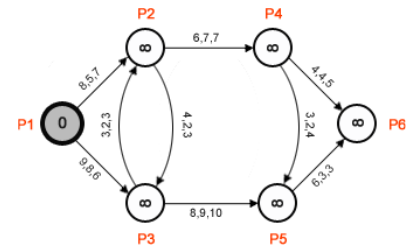
\includegraphics[width=.50\textwidth]{chapters/fig/leo2.png}
\caption{Processo de determinação de caminho mínimo - Parte 1}
\label{fig:leo2}
\end{figure}

\begin{table}[htbp]
	\centering
	\begin{tabular}{l l l l}
	\toprule
	Vértice & PERM & Distância & Predecessor\\
	\midrule
	P1 & Sim & 0 & - \\
	P2 & Não & $\infty$ & - \\
	P3 & Não & $\infty$ & - \\
	P4 & Não & $\infty$ & - \\
	P5 & Não & $\infty$ & - \\
	P6 & Não & $\infty$ & - \\
	\bottomrule
	\end{tabular}
\caption{Processo de determinação de caminho mínimo - Parte 1}
 \label{tab:leotab1}
\end{table}
\FloatBarrier

A partir de P1 consulta-se os vértices adjacentes a ele, que são P2 e P3. Para todos os vértices
adjacentes denonimados $s$, calcula-se o pseudocódigo da figura \ref{fig:diMod}.

\fbox{\begin{minipage}{70ex}
\vspace*{-1mm} \phantom{} \hspace{3ex} {\bf Se} dist[s] > dist[d]\ + peso(d,s)\\
\vspace*{-1mm} \phantom{} \hspace{6ex} dist[s] = dist[d]\ + peso(d,s)\\
\vspace*{-1mm} \phantom{} \hspace{6ex} path[s] = s\\
\vspace*{-1mm} \phantom{} \hspace{3ex} {\bf Fim Se}\\
\end{minipage}}
\begin{figure}[htbp]
\centering
\caption{Dijkstra Modificado - Trecho aplicado a vértices adjacentes}
\label{fig:diMod}
\end{figure}
\FloatBarrier

\begin{figure}[htbp]
\centering
 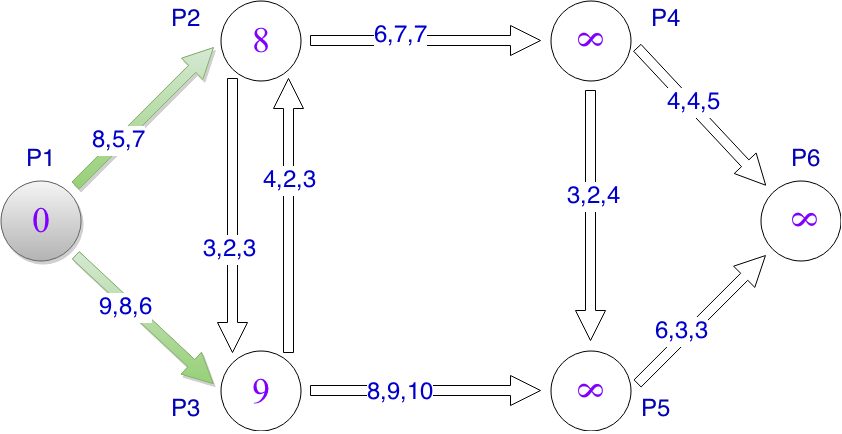
\includegraphics[width=.50\textwidth]{chapters/fig/leo3.png}
\caption{Processo de determinação de caminho mínimo - Parte 2}
\label{fig:leo3}
\end{figure}

\begin{table}[htbp]
	\centering
	\begin{tabular}{l l l l}
	\toprule
	Vértice & PERM & Distância & Predecessor\\
	\midrule
	P1 & Sim & 0 & - \\
	P2 & Não & 8 & P1 \\
	P3 & Não & 9 & P1 \\
	P4 & Não & $\infty$ & - \\
	P5 & Não & $\infty$ & - \\
	P6 & Não & $\infty$ & - \\
	\bottomrule
	\end{tabular}
\caption{Processo de determinação de caminho mínimo - Parte 2}
 \label{tab:leotab2}
\end{table}
\FloatBarrier

P2 é selecionado de PERM, pois possui a menor distância dist[x] = 8. Então inclui-se x em PERM e consulta-se
seus vértices adjacentes, que no caso são P3 e P4.

\begin{figure}[htbp]
\centering
 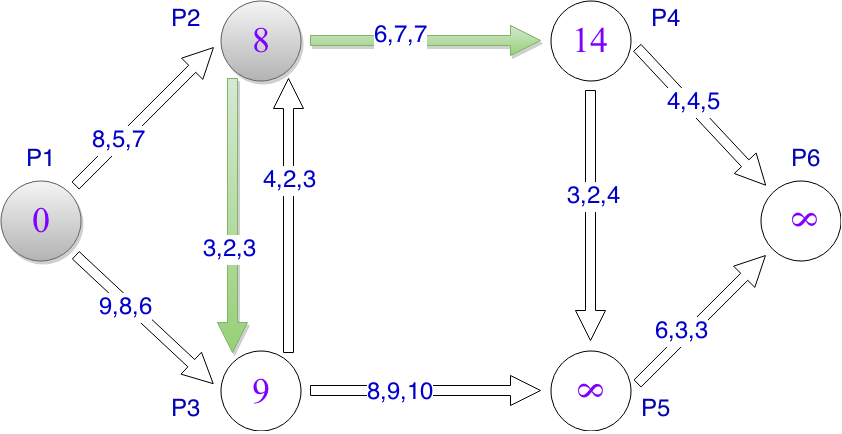
\includegraphics[width=.50\textwidth]{chapters/fig/leo4.png}
\caption{Processo de determinação de caminho mínimo - Parte 3}
\label{fig:leo4}
\end{figure}
\FloatBarrier

\begin{table}[htbp]
	\centering
	\begin{tabular}{l l l l}
	\toprule
	Vértice & PERM & Distância & Predecessor\\
	\midrule
	P1 & Sim & 0 & - \\
	P2 & Sim & 8 & P1 \\
	P3 & Não & 9 & P1 \\
	P4 & Não & 14 & P2 \\
	P5 & Não & $\infty$ & - \\
	P6 & Não & $\infty$ & - \\
	\bottomrule
	\end{tabular}
\caption{Processo de determinação de caminho mínimo - Parte 3}
 \label{tab:leotab3}
\end{table}
\FloatBarrier

\begin{figure}[htbp]
\centering
 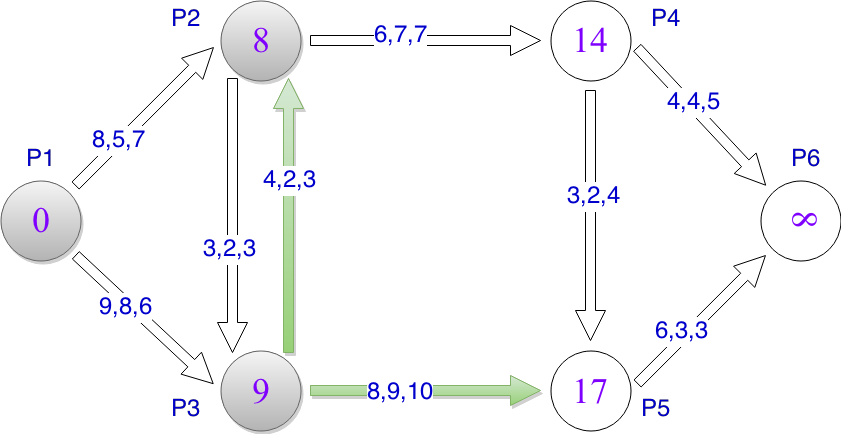
\includegraphics[width=.50\textwidth]{chapters/fig/leo5.png}
\caption{Processo de determinação de caminho mínimo - Parte 4}
\label{fig:leo5}
\end{figure}

\begin{table}[htbp]
	\centering
	\begin{tabular}{l l l l}
	\toprule
	Vértice & PERM & Distância & Predecessor\\
	\midrule
	P1 & Sim & 0 & - \\
	P2 & Sim & 8 & P1 \\
	P3 & Sim & 9 & P1 \\
	P4 & Não & 14 & P2 \\
	P5 & Não & 17 & P3 \\
	P6 & Não & $\infty$ & - \\
	\bottomrule
	\end{tabular}
\caption{Processo de determinação de caminho mínimo - Parte 4}
 \label{tab:leotab4}
\end{table}
\FloatBarrier

Ao selecionar o vértice P4, não pertencente a PERM, o intervalo de previsão é ultrapassado
de 10 minutos. Logo, é utilizada a segunda posição do vetor de custos $t + 2$. O custo do trajeto até
o vértice P5 pelo P4 é menor do que o custo atual por P3, logo atualiza-se seu peso e predecessor
para 16 e P4 respectivamente.
\FloatBarrier
\begin{figure}[htbp]
\centering
 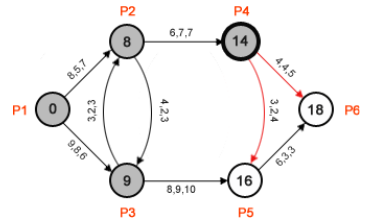
\includegraphics[width=.50\textwidth]{chapters/fig/leo6.png}
\caption{Processo de determinação de caminho mínimo - Parte 5}
\label{fig:leo6}
\end{figure}

\begin{table}[htbp]
	\centering
	\begin{tabular}{l l l l}
	\toprule
	Vértice & PERM & Distância & Predecessor\\
	\midrule
	P1 & Sim & 0 & - \\
	P2 & Sim & 8 & P1 \\
	P3 & Sim & 9 & P1 \\
	P4 & Sim & 14 & P2 \\
	P5 & Não & 16 & P4 \\
	P6 & Não & 18 & P4 \\
	\bottomrule
	\end{tabular}
\caption{Processo de determinação de caminho mínimo - Parte 5}
 \label{tab:leotab5}
\end{table}

P5 é adicionado a PERM e seu único vértice adjacente é P6. Logo temos:
\FloatBarrier
\begin{figure}[htbp]
\centering
 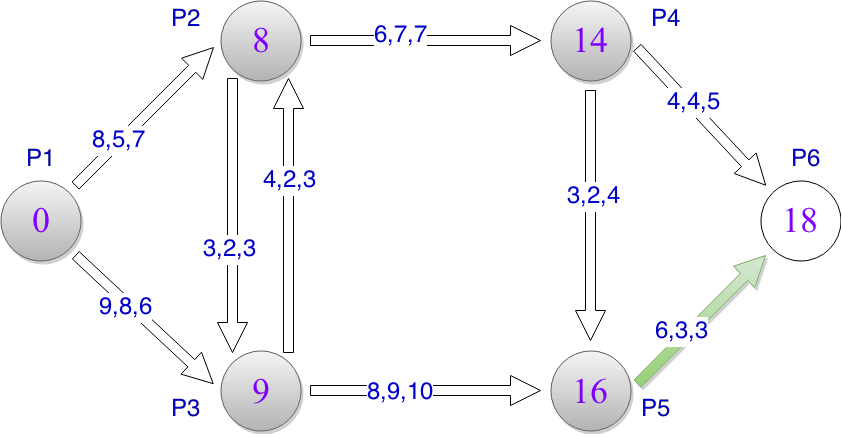
\includegraphics[width=.50\textwidth]{chapters/fig/leo7.png}
\caption{Processo de determinação de caminho mínimo - Parte 6}
\label{fig:leo7}
\end{figure}

\begin{table}[htbp]
	\centering
	\begin{tabular}{l l l l}
	\toprule
	Vértice & PERM & Distância & Predecessor\\
	\midrule
	P1 & Sim & 0 & - \\
	P2 & Sim & 8 & P1 \\
	P3 & Sim & 9 & P1 \\
	P4 & Sim & 14 & P2 \\
	P5 & Sim & 16 & P4 \\
	P6 & Sim & 18 & P4 \\
	\bottomrule
	\end{tabular}
\caption{Processo de determinação de caminho mínimo - Parte 6}
 \label{tab:leotab5}
\end{table}
\FloatBarrier

E finalmente temos a figura \ref{fig:leo8}, pois P6 não possui vértice adjacente. Logo, o 
tempo para percorrer o caminho mínimo passando por P1, P2, P4 e P6 é 18 minutos.

\begin{figure}[htbp]
\centering
 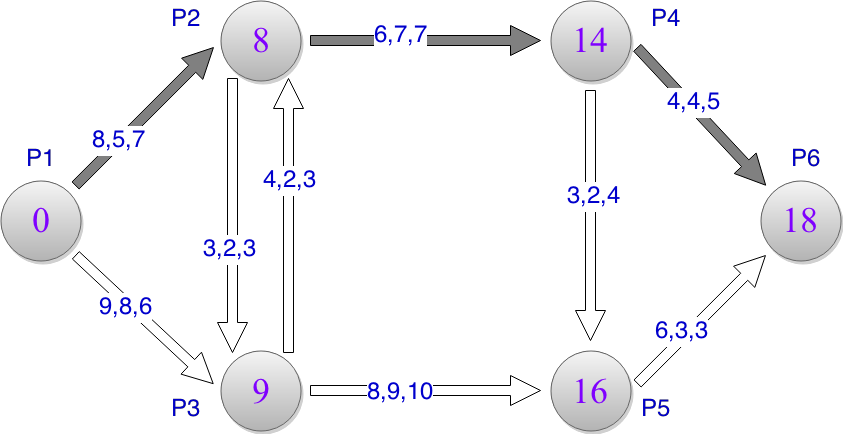
\includegraphics[width=.50\textwidth]{chapters/fig/leo8.png}
\caption{Processo de determinação de caminho mínimo - Parte 7}
\label{fig:leo8}
\end{figure}
\FloatBarrier

A presente pesquisa resolve o mesmo problema utilizando o Algoritmo de Dijkstra com Radix Heap para Grafos Dinâmicos.
Foram implementados dois algoritmos nesse contexto: o primeiro segue a mesma abordagem do Dijkstra Modificado \cite{leonard},
em relação a mudança do tempo de previsão ao exceder 10 minutos; e o segundo altera o intervalo de previsão quando o valor
do custo do vértice acrescido do valor do custo da aresta adjacente for superior a 10. Os dois usados em conjunto indicam
um intervalo de limite inferior e superior para determinação do caminho mínimo.

Os dois algoritmos utilizam um vetor de custos composto pelo tempo médio das passagens dos veículos, em intervalos
de 10 minutos ao longo do dia, numa determinada ligação ou aresta. Por exemplo, entre 12 horas e 12 horas e 10 minutos um
veículo demora em média 2 minutos para percorrer a aresta, entre 12 horas e 10 minutos e 12h e 20 minutos ele demora 3 minutos
para percorrer a mesma aresta, e assim por diante. Os dados do vetor de custo são armazenados em um arquivo no formato JSON
como mostra a figura \ref{fig:tabelajson}. Cada aresta possui um vetor de tamanho 24 para representar as horas, e cada elemento
do vetor possui um vetor de tamanho 6 para representar os intervalos de 10 minutos ao longo de 1 hora.
\begin{center}
  \line(1,0){450}
\end{center}
\lstinputlisting[language=Java]{chapters/tabela.json}
\begin{figure}[htbp]
  \begin{center}
    \line(1,0){450}
  \end{center}
  \centering
  \caption{Estrutura JSON usada pelo vetor de custos}
  \label{fig:tabelajson}
\end{figure}
\FloatBarrier

A mudança de intervalo de previsão do segundo algoritmo segue o seguinte exemplo: se o tempo parcial até um determinado 
ponto somado ao custo de travessia da aresta adjacente for de 8 minutos, então é utilizado para o próximo cálculo o tempo
de previsão no intervalo $t + 1$, mas se a soma for de 13 minutos, logo o período de previsão é ultrapassado, e com isso
utiliza-se $t + 2$ para o cálculo do próximo trajeto. Se a soma estiver entre 20 e 30 minutos utiliza-se o intervalo
$t + 3$, entre 30 e 40 minutos $t + 4$, e assim por diante.
A figura \ref{fig:radixMod} apresenta o pseudocódigo do algoritmo em questão.
\FloatBarrier
\fbox{\begin{minipage}{70ex}
\noindent \phantom{} \hspace{0ex} {\bf Dijkstra com Radix Heap em Grafos Dinâmicos}\\
\vspace*{-1mm} \phantom{} \hspace{3ex} buckets = [];\\
\vspace*{-1mm} \phantom{} \hspace{3ex} Inicializa o rótulo de distância dos vértices\\
\vspace*{-1mm} \phantom{} \hspace{3ex} {\bf Para} i = 1 até i < vertices.length\\
\vspace*{-1mm} \phantom{} \hspace{6ex} vertices[i].rotulo = MAXINT\\
\vspace*{-1mm} \phantom{} \hspace{3ex} {\bf Fim Para}\\
\vspace*{-1mm} \phantom{} \hspace{3ex} Inicializa os buckets e seus intervalos\\
\vspace*{-1mm} \phantom{} \hspace{3ex} {\bf Para} i = 0 até i < buckets.length\\
\vspace*{-1mm} \phantom{} \hspace{6ex} iniBucket = $2^{k - 1}$\\
\vspace*{-1mm} \phantom{} \hspace{6ex} fimBucket = $2^k - 1$\\
\vspace*{-1mm} \phantom{} \hspace{6ex} adiciona Bucket(iniBucket, fimBucket) a buckets\\
\vspace*{-1mm} \phantom{} \hspace{3ex} {\bf Fim Para}\\
\vspace*{-1mm} \phantom{} \hspace{3ex} Insere os vértices dentro dos buckets correspondentes\\
\vspace*{-1mm} \phantom{} \hspace{3ex} {\bf Enquanto} todos os vértices não forem rotulados permanentemente\\
\vspace*{-1mm} \phantom{} \hspace{6ex} menorBucket = menor bucket não vazio\\
\vspace*{-1mm} \phantom{} \hspace{6ex} {\bf Se} (o menorBucket tem largura = 1 || menorBucket.size = 1)\\
\vspace*{-1mm} \phantom{} \hspace{9ex} verticeSelecionado = vértice do menorBucket\\
\vspace*{-1mm} \phantom{} \hspace{9ex} {\bf Se} verticeSelecionado não foi rotulado permanentemente\\
\vspace*{-1mm} \phantom{} \hspace{12ex} {\bf Para} i = 0 até i < verticeSelecionado.getArcos().size\\
\vspace*{-1mm} \phantom{} \hspace{15ex} Atualiza o rótulo do vérticeDestino\\
\vspace*{-1mm} \phantom{} \hspace{15ex} Insere o vértice no bucket correspondente\\
\vspace*{-1mm} \phantom{} \hspace{12ex} {\bf Fim Para}\\
\vspace*{-1mm} \phantom{} \hspace{9ex} {\bf Fim Se}\\
\vspace*{-1mm} \phantom{} \hspace{9ex} Remove do bucket o verticeSelecionado\\
\vspace*{-1mm} \phantom{} \hspace{9ex} Marca o rótulo verticeSelecionado permanentemente\\
\vspace*{-1mm} \phantom{} \hspace{6ex} {\bf Fim Se}\\
\vspace*{-1mm} \phantom{} \hspace{6ex} {\bf Senão}\\
\vspace*{-1mm} \phantom{} \hspace{9ex} Recalcula o intervalo dos buckets\\
\vspace*{-1mm} \phantom{} \hspace{9ex} Redistribui os vertices\\
\vspace*{-1mm} \phantom{} \hspace{3ex} {\bf Fim Enquanto}\\
\vspace*{-1mm} \phantom{} \hspace{0ex} {\bf Fim RadixHeap}\\
\end{minipage}}
\begin{figure}[htbp]
\centering
\caption{Dijkstra com Radix Heap}
\label{fig:radixMod}
\end{figure}

A seguir, é apresentado o funcionamento do algoritmo utilizando o mesmo grafo da figura \ref{fig:leo1}
e o mesmo ponto de origem. Para determinar o caminho mínimo, cada vértice armazena o identificador do vértice anterior.
O algoritmo utiliza ``buckets'' para armazenar os vértices de acordo com seus rótulos.
Inicialmente, os rótulos de todos os vértices recebem um custo de valor tendendo ao infinito exceto P1,
que possui custo 0, da mesma forma que a figura \ref{fig:leo2}. A figura \ref{fig:buckets} exibe a disposição dos vértices em seus
respectivos ``buckets''.

\begin{figure}[htbp]
\centering
 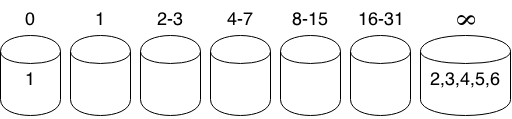
\includegraphics[width=.50\textwidth]{chapters/fig/buckets.png}
\caption{Disposição dos vértices nos buckets}
\label{fig:buckets}
\end{figure}
\FloatBarrier

Após consultar os vértices adjacentes a P1, que são P2 e P3, o pseudocódigo da figura \ref{fig:janelatemporal}
é executado e o mesmo resultado da figura \ref{fig:leo3} é encontrado. Em seguida, os ``buckets'' são atualizados
como mostra a figura \ref{fig:buckets1}.

\fbox{\begin{minipage}{70ex}
\vspace*{-1mm} \phantom{} \hspace{3ex} custoAresta = horário até o momento\\
\vspace*{-1mm} \phantom{} \hspace{3ex} {\bf Se} custoAresta + custoVerticeSelecionado > janelaTemporalAtual\\
\vspace*{-1mm} \phantom{} \hspace{6ex} custoAresta = tempo de previsão do próximo intervalo\\
\vspace*{-1mm} \phantom{} \hspace{3ex} {\bf Fim Se}\\
\vspace*{-1mm} \phantom{} \hspace{3ex} {\bf Se} custoAresta + custoVerticeSelecionado < rótulo do verticeDestino\\
\vspace*{-1mm} \phantom{} \hspace{6ex} custoAresta = custoAresta + custoVerticeSelecionado\\
\vspace*{-1mm} \phantom{} \hspace{6ex} identificador do verticeDestino recebe identificador vértice anterior\\
\vspace*{-1mm} \phantom{} \hspace{3ex} {\bf Fim Se}\\
\vspace*{-1mm} \phantom{} \hspace{3ex} {\bf Senão}\\
\vspace*{-1mm} \phantom{} \hspace{6ex} custoAresta = rótulo do verticeDestino\\
\vspace*{-1mm} \phantom{} \hspace{3ex} rótulo do verticeDestino = custoAresta\\
\end{minipage}}
\begin{figure}[htbp]
\centering
\caption{Radix Heap - Pseudocódigo para rotular os vértices adjacentes}
\label{fig:janelatemporal}
\end{figure}
\FloatBarrier

\begin{figure}[htbp]
\centering
 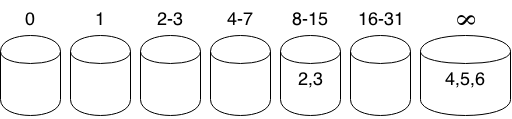
\includegraphics[width=.50\textwidth]{chapters/fig/buckets1.png}
\caption{Disposição dos vértices nos buckets - Parte 1}
\label{fig:buckets1}
\end{figure}
\FloatBarrier

Como o menor ``bucket'' não tem largura igual a 1 e possui mais de 1 elemento, o intervalo dos ``buckets''
é atualizado:

\begin{figure}[htbp]
\centering
 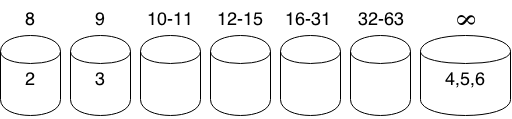
\includegraphics[width=.50\textwidth]{chapters/fig/buckets2.png}
\caption{Disposição dos vértices nos buckets - Parte 2}
\label{fig:buckets2}
\end{figure}
\FloatBarrier

O vértice P2 é selecionado do menor ``bucket'' e em seguida consulta-se seus vértices adjacentes, que são P3 e P4.
O intervalo de previsão é ultrapassado ao somar o rótulo de P2 com o custo da aresta, que segue até P3, no intervalo $t + 1$. Logo, 
é utilizado a próxima posição do vetor de custos, que é $t + 2$. As figuras \ref{fig:limitesup1} e \ref{fig:buckets3} exibem o resultado.

\begin{figure}[htbp]
\centering
 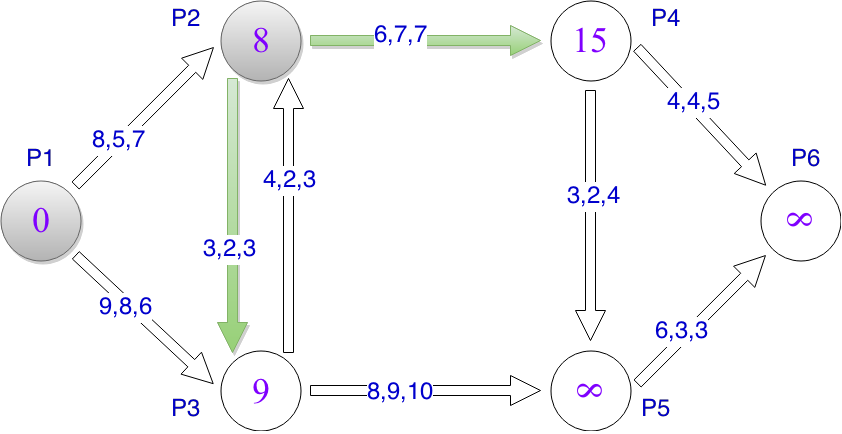
\includegraphics[width=.50\textwidth]{chapters/fig/limitesup1.png}
\caption{Radix Heap - Parte 1}
\label{fig:limitesup1}
\end{figure}

\begin{figure}[htbp]
\centering
 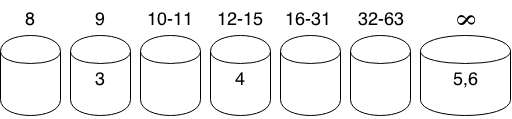
\includegraphics[width=.50\textwidth]{chapters/fig/buckets3.png}
\caption{Disposição dos vértices nos buckets - Parte 3}
\label{fig:buckets3}
\end{figure}
\FloatBarrier

Em seguida, são exibidos os próximos passos até chegar no resultado final.

\begin{figure}[htbp]
\centering
 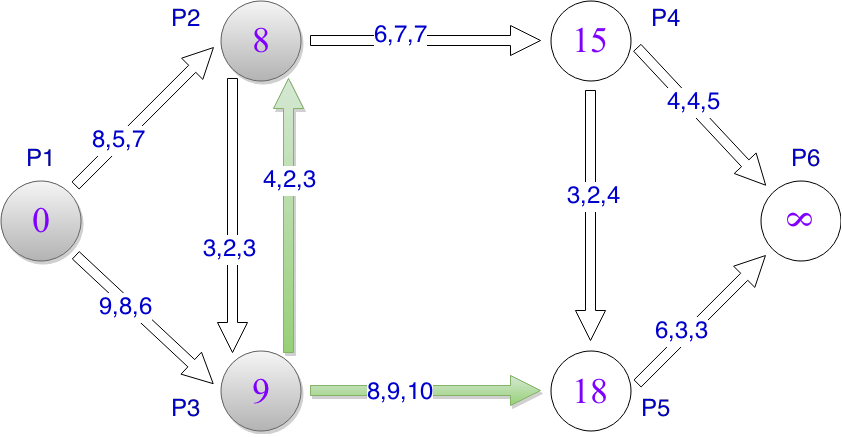
\includegraphics[width=.50\textwidth]{chapters/fig/limitesup2.png}
\caption{Radix Heap - Parte 2}
\label{fig:limitesup2}
\end{figure}

\begin{figure}[htbp]
\centering
 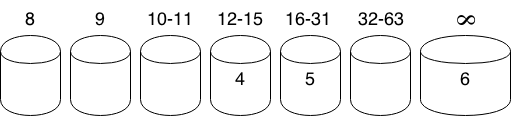
\includegraphics[width=.50\textwidth]{chapters/fig/buckets4.png}
\caption{Disposição dos vértices nos buckets - Parte 4}
\label{fig:buckets4}
\end{figure}

\begin{figure}[htbp]
\centering
 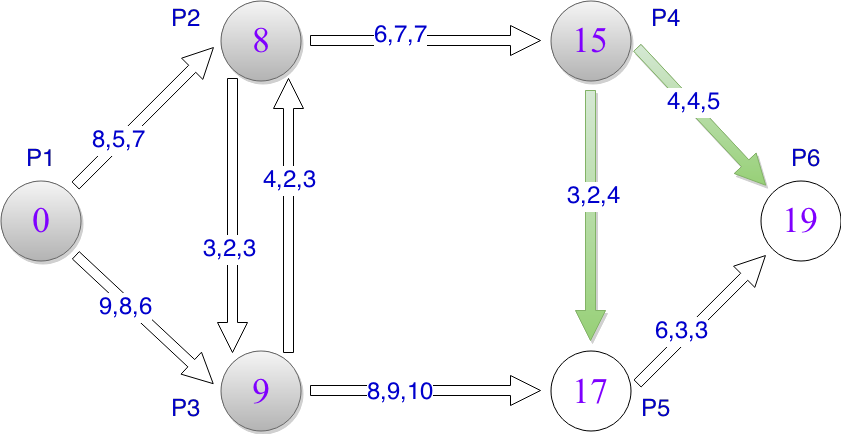
\includegraphics[width=.50\textwidth]{chapters/fig/limitesup3.png}
\caption{Radix Heap - Parte 3}
\label{fig:limitesup3}
\end{figure}

\begin{figure}[htbp]
\centering
 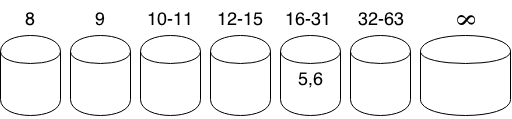
\includegraphics[width=.50\textwidth]{chapters/fig/buckets5.png}
\caption{Disposição dos vértices nos buckets - Parte 5}
\label{fig:buckets5}
\end{figure}
\FloatBarrier

Novamente o intervalo dos ``buckets'' é atualizado e P5 é selecionado.

\begin{figure}[htbp]
\centering
 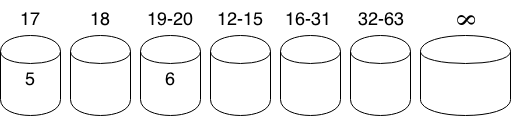
\includegraphics[width=.50\textwidth]{chapters/fig/buckets6.png}
\caption{Disposição dos vértices nos buckets - Parte 6}
\label{fig:buckets6}
\end{figure}

\begin{figure}[htbp]
\centering
 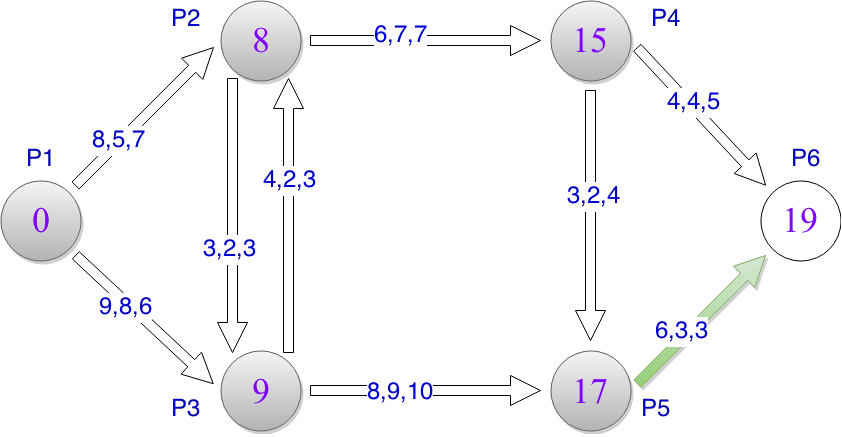
\includegraphics[width=.50\textwidth]{chapters/fig/limitesup4.png}
\caption{Radix Heap - Parte 4}
\label{fig:limitesup4}
\end{figure}

\begin{figure}[htbp]
\centering
 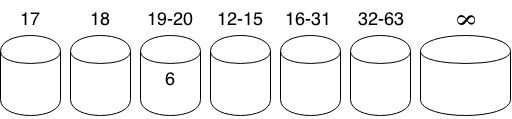
\includegraphics[width=.50\textwidth]{chapters/fig/buckets7.png}
\caption{Disposição dos vértices nos buckets - Parte 7}
\label{fig:buckets7}
\end{figure}
\FloatBarrier

Finalmente, P6 é selecionado, mas como não possui vértices adjcentes, o caminho mínimo é definido passando
pelos vértices P1, P2, P4 e P6 com tempo de percurso de 19 minutos, como mosta a figura \ref{fig:limitesup5}.

\begin{figure}[htbp]
\centering
 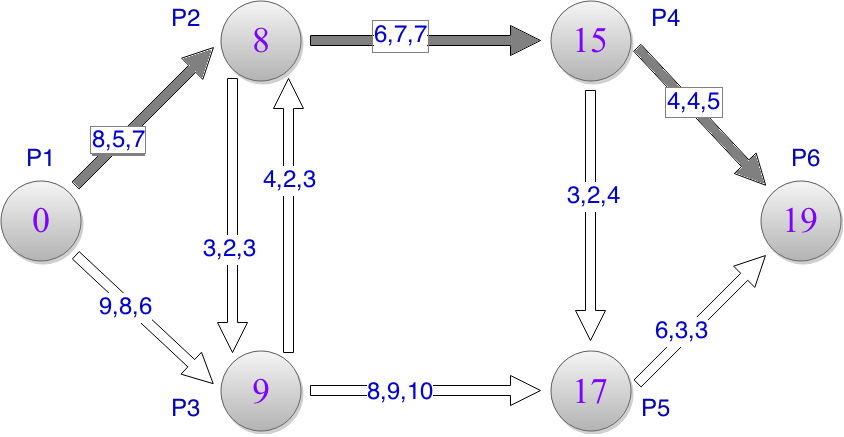
\includegraphics[width=.50\textwidth]{chapters/fig/limitesup5.png}
\caption{Radix Heap - Parte 5}
\label{fig:limitesup5}
\end{figure}
\FloatBarrier

O exemplo da figura \ref{fig:intervalo} exibe a resolução dos caminhos mínimos de dois grafos de vetor de custo distintos,
usando os dois algoritmos implementados nesta pesquisa. 
\begin{figure}[htbp]
\centering
 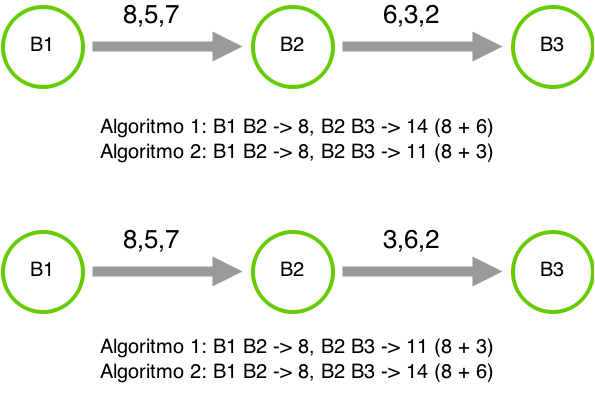
\includegraphics[width=.60\textwidth]{chapters/fig/intervalo.png}
\caption{Grafo exemplo para indicar o Intervalo de Previsão}
\label{fig:intervalo}
\end{figure}
\FloatBarrier

\subsubsection{Topologia Dinâmica e Atributos Estáticos}
Esse algoritmo não foi implementado e segue a estrutura apresentada na seção \ref{subsec:topdinatribest},
onde vértices e arestas podem mudar ao longo do tempo e seus atributos são constantes. A 
figura \ref{fig:pathtopdyn} apresenta essa estrutura:

\begin{figure}[htbp]
\centering
 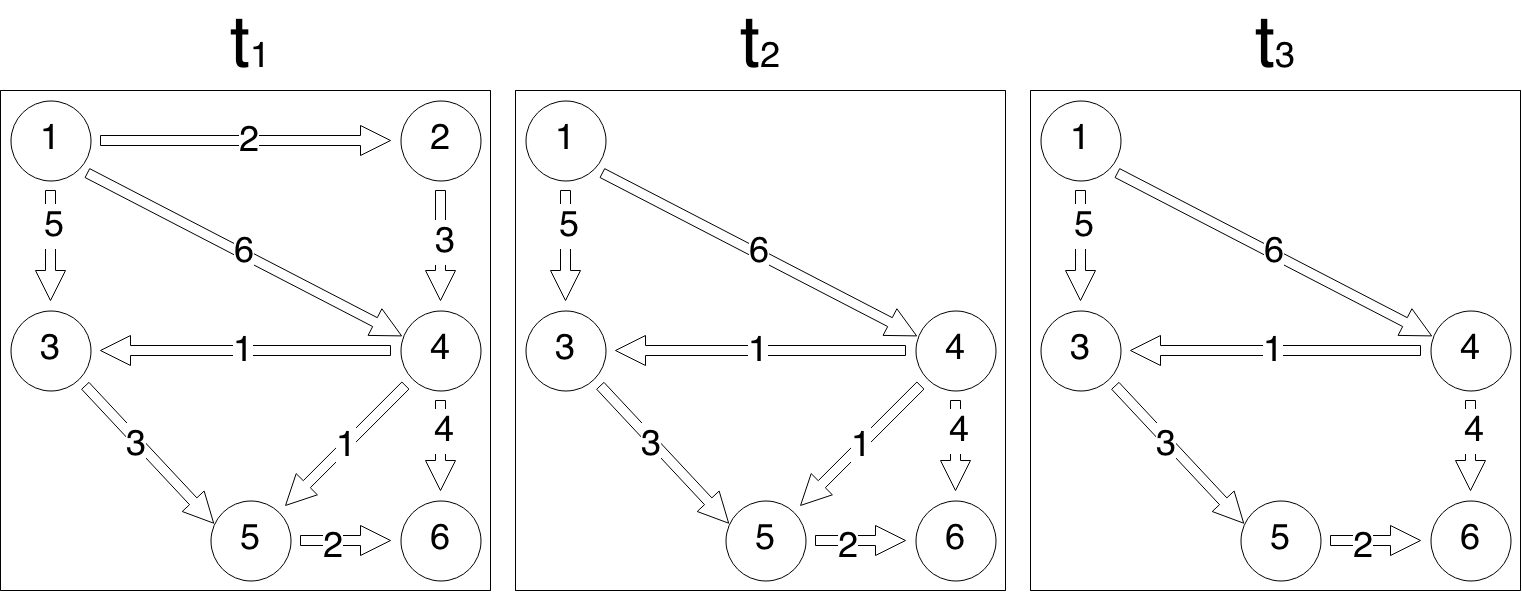
\includegraphics[width=.80\textwidth]{chapters/fig/pathtopdyn.png}
\caption{Caminho Mínimo - Topologia Dinâmica e Atributos Estáticos}
\label{fig:pathtopdyn}
\end{figure}
\FloatBarrier
O exemplo utiliza pontos representados através do grafo G(N=\{P1, P2, P3, P4, P5, P6\}, A), onde o 
ponto de partida é P1 e o destino o ponto P6. No instante $t_1$ é possível observar vários caminhos
até chegar ao objetivo. Já no instante $t_2$ o vértice P2 foi removido, e em $t_3$ a aresta que começa em
P4 e vai até P5 é removida, e com isso reduzindo as possibilidades de chegar a P6. Diante disso,
se faz necessário conhecer o tempo inicial e final de cada vértice e aresta para chegar a P6.

\subsubsection{Topologia Dinâmica e Atributos Dinâmicos}
Essa seção resolve o problema apresentado na seção \ref{subsec:limitesuperior} utilizando o Algoritmo de
Dijkstra com Radix Heap seguindo a estrutura da seção \ref{subsec:topdinatridin}.

Ao executar o exemplo da figura \ref{fig:leo1}, com o mesmo vetor de custo e ponto de origem, tem-se
os vértices adjacentes P2 e P3. Ao atualizar o rótulo dos vértices adjacentes, é necessário executar o mesmo
pseudocódigo apresentado na figura \ref{fig:janelatemporal}. Além disso, é levado em consideração o tempo
inicial e final dos vértices e arestas para determinar o caminho mínimo. Para isso,
verifica-se as seguintes questões:
\begin{itemize}
\item Se a aresta já existe, ou seja, se o tempo inicial dela é menor que o horário atual;
\item Se a aresta existirá durante o tempo de travessia, que correspondente ao custo dela no intervalo de previsão;
\item Se os vértices origem e destino existirão durante durante a travessia.
\end{itemize}
\FloatBarrier

A figura abaixo exibe o tempo de existência de cada elemento do grafo:
\begin{center}
  \line(1,0){450}
\end{center}
\lstinputlisting[language=Java]{chapters/datatime.json}
\begin{figure}[htbp]
  \begin{center}
    \line(1,0){450}
  \end{center}
  \centering
  \caption{Estrutura JSON do tempo de existência dos vértices e arestas}
  \label{fig:datatime}
\end{figure}
\FloatBarrier

Tomando os vértices adjacentes a P1, observa-se o grafo da figura \ref{fig:dyndyn1}, onde as arestas
que ligam P1 a P2 e P4 a P5 ainda não existem.

\begin{figure}[htbp]
\centering
 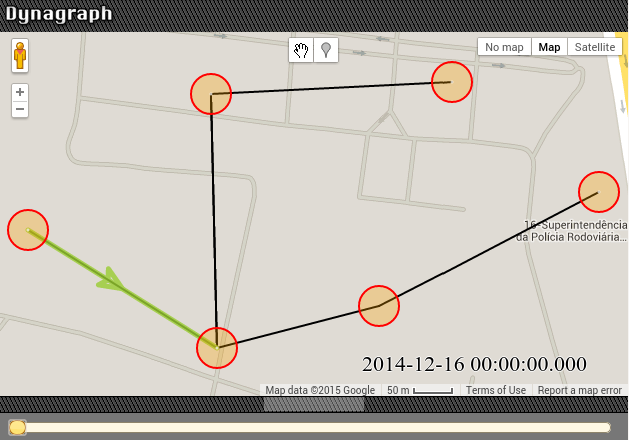
\includegraphics[width=.55\textwidth]{chapters/fig/dyndyn1.png}
\caption{Radix Heap Dinâmico - Parte 1}
\label{fig:dyndyn1}
\end{figure}
\FloatBarrier

A seguir, é apresentada a sequência de instantes utilizando o dynagraph após resolução do algoritmo.

\begin{figure}[htbp]
\centering
 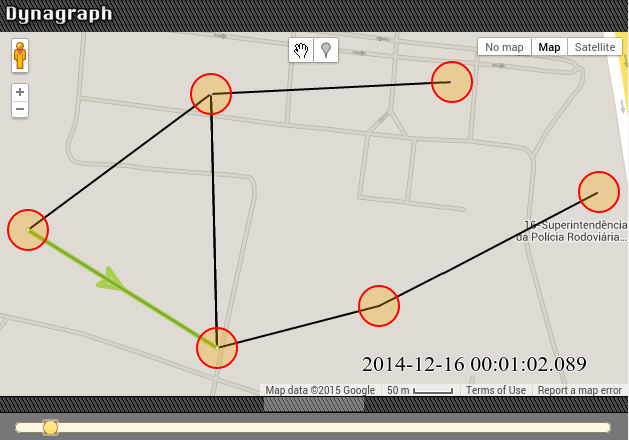
\includegraphics[width=.45\textwidth]{chapters/fig/dyndyn2.png}
 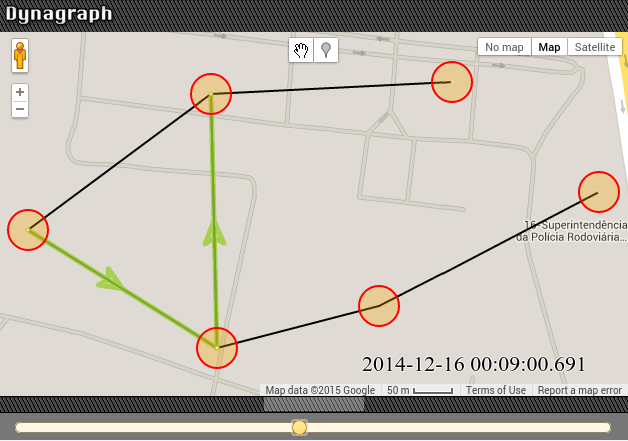
\includegraphics[width=.45\textwidth]{chapters/fig/dyndyn3.png}
\caption{Radix Heap Dinâmico - Parte 2 e 3}
\label{fig:dyndyn2}
\end{figure}

\begin{figure}[htbp]
\centering
 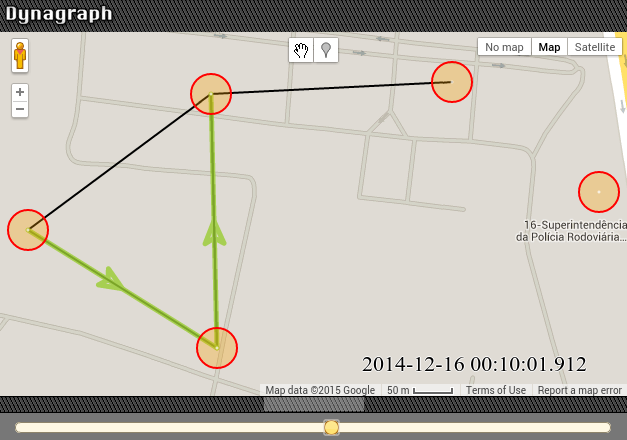
\includegraphics[width=.45\textwidth]{chapters/fig/dyndyn4.png}
 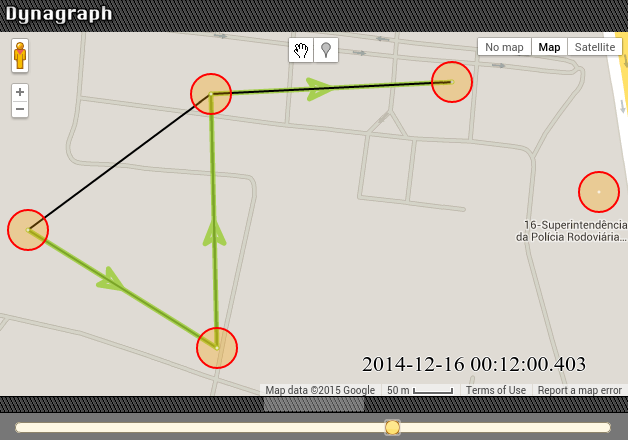
\includegraphics[width=.45\textwidth]{chapters/fig/dyndyn5.png}
\caption{Radix Heap Dinâmico - Parte 4 e 5}
\label{fig:dyndyn3}
\end{figure}


\begin{figure}[htbp]
\centering
 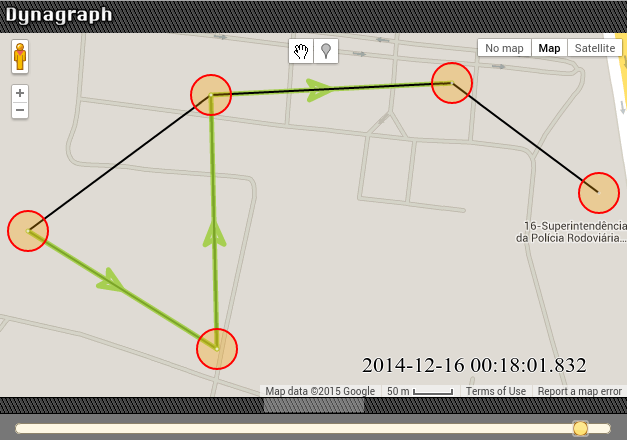
\includegraphics[width=.45\textwidth]{chapters/fig/dyndyn6.png}
 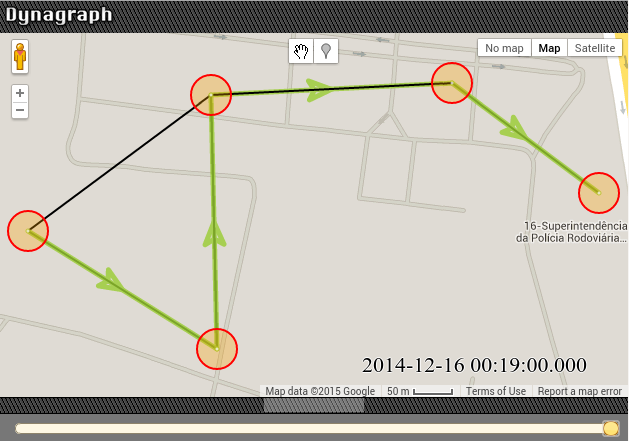
\includegraphics[width=.45\textwidth]{chapters/fig/dyndyn7.png}
\caption{Radix Heap Dinâmico - Parte 6 e 7}
\label{fig:dyndyn4}
\end{figure}














